\subsection{Tests de correctitud}

Para verificar el correcto funcionamiento del algoritmo tomamos distintas instancias del problema:

\begin{figure}[H]
 \centering
  \subfloat[3 fábricas y 6 clientes.]{
   \label{}
    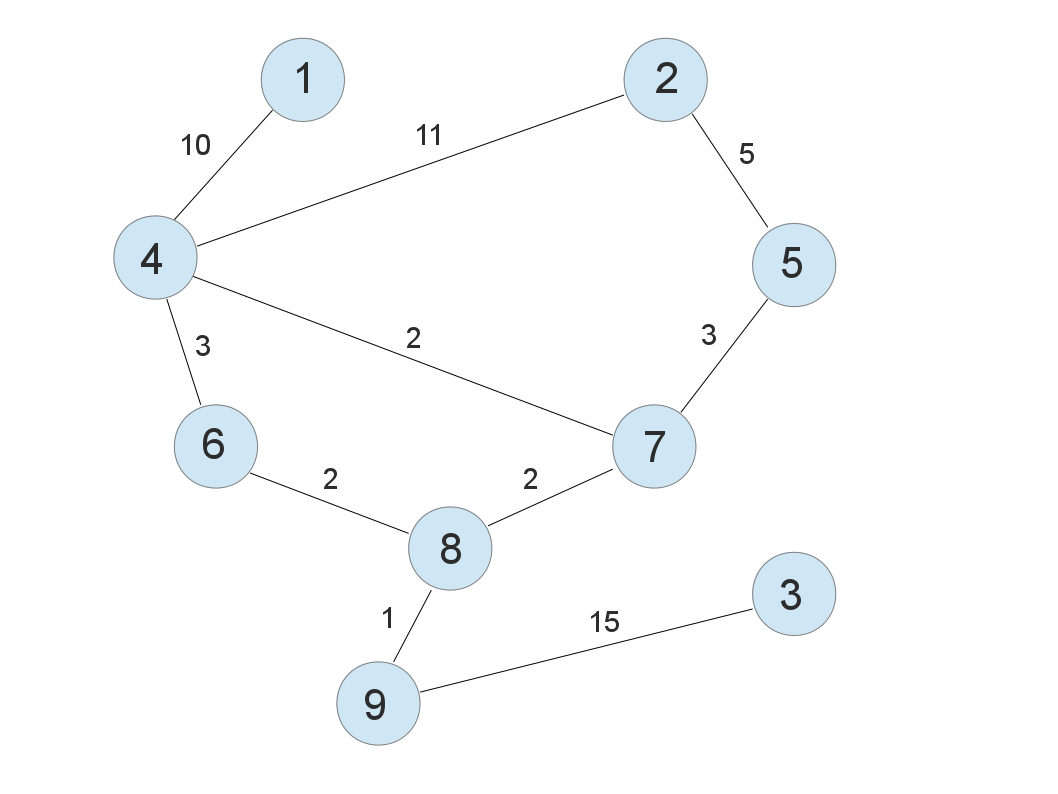
\includegraphics[scale=0.3]{ej3/imgs/graph_test1.png}}
  \subfloat[2 fábricas y 2 clientes.]{
   \label{}
    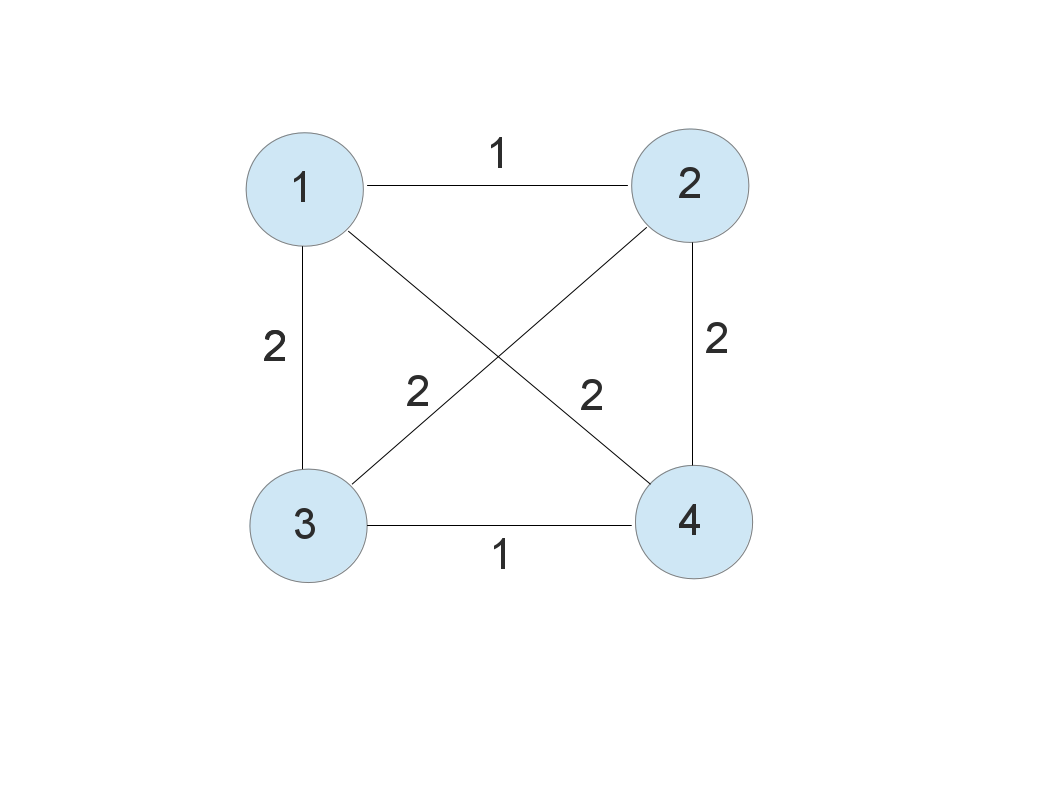
\includegraphics[scale=0.3]{ej3/imgs/graph_test2.png}}
  \subfloat[2 fábricas y 2 clientes.]{
   \label{}
    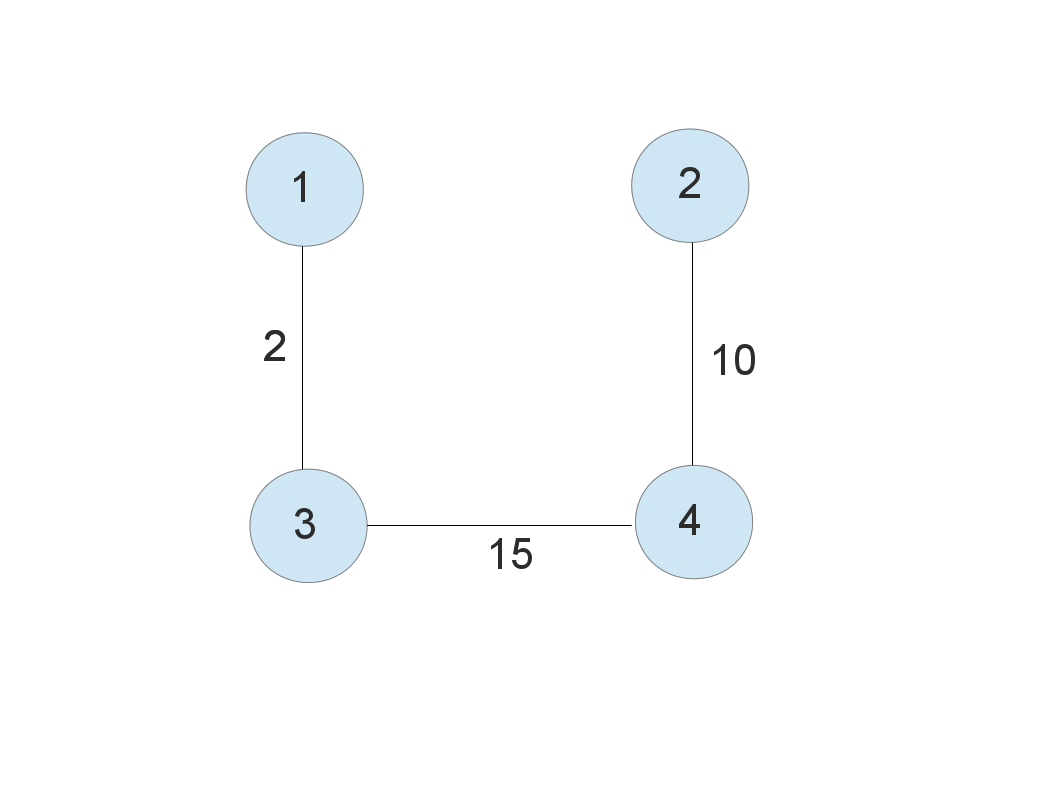
\includegraphics[scale=0.3]{ej3/imgs/graph_test3.png}}
  \subfloat[3 fábricas y 6 clientes.]{
   \label{}
    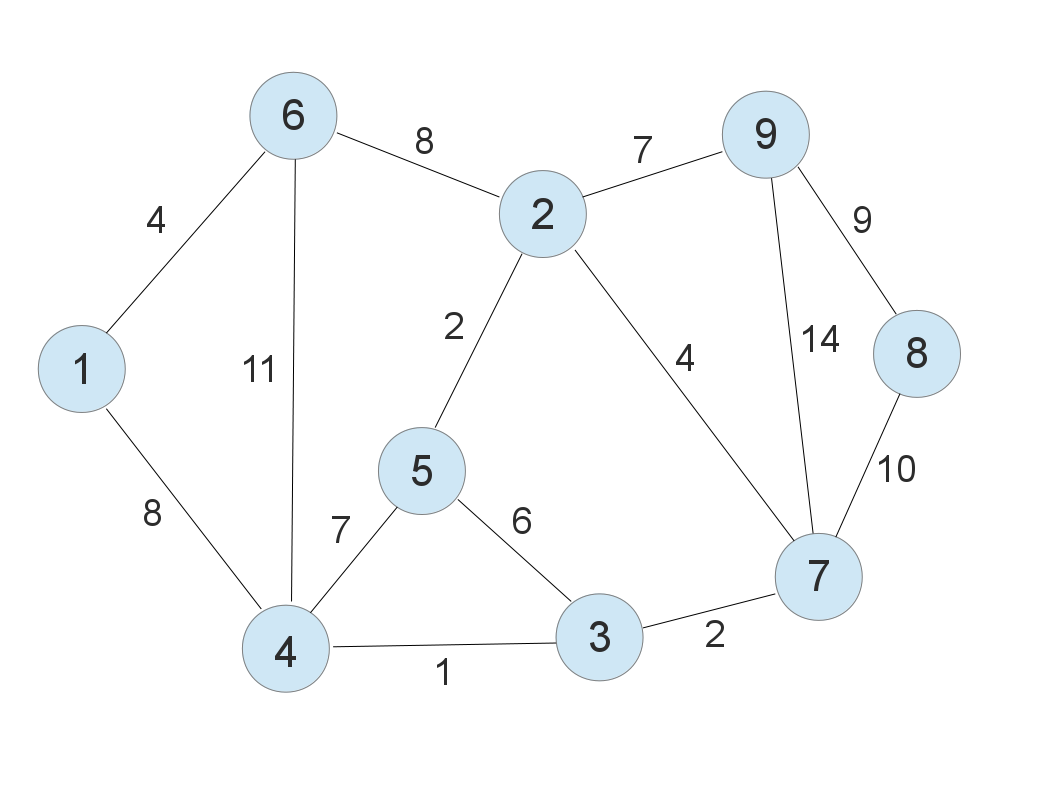
\includegraphics[scale=0.3]{ej3/imgs/graph_test4.png}}
 \caption{Casos de prueba}
 \label{}
\end{figure}

Utilizamos estos casos de prueba para observar que efectivamente formaba bosques de AGM cuando la solución lo requería y que además no usara aristas que conectaran dos fábricas entre si. Las soluciones obtenidas fueron:

\begin{figure}[H]
 \centering
  \subfloat[Costo total: 15]{
   \label{}
    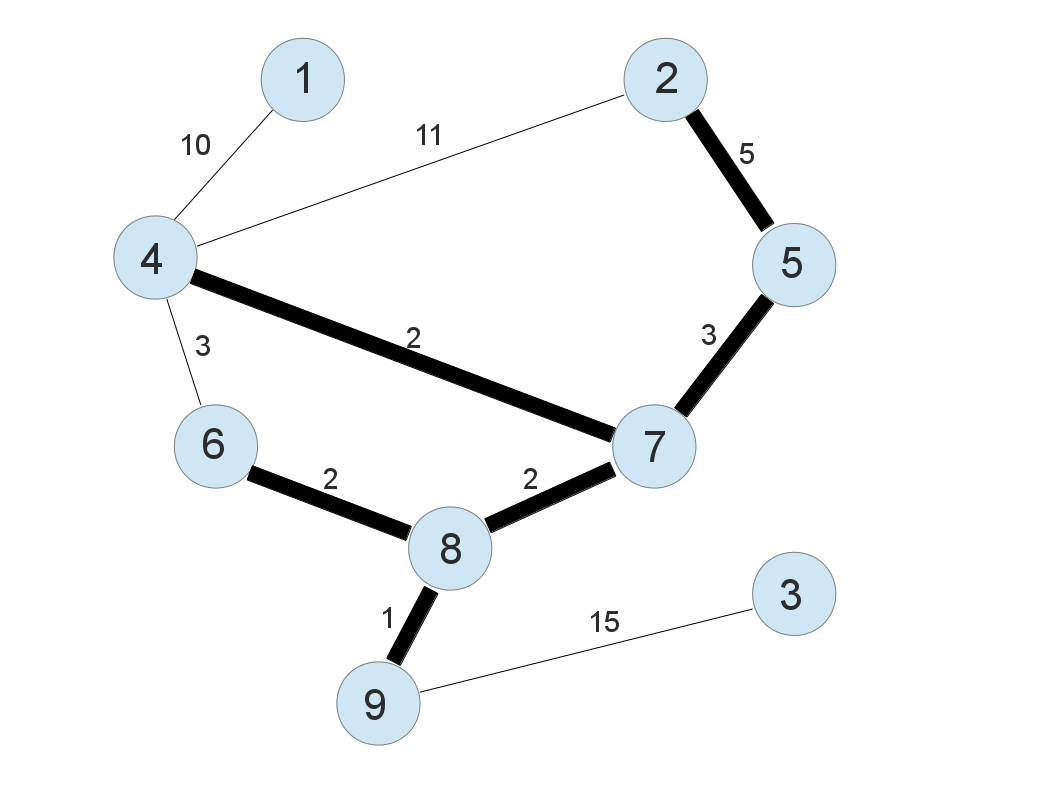
\includegraphics[scale=0.3]{ej3/imgs/graph_test1_sol.png}}
  \subfloat[Costo total: 3]{
   \label{}
    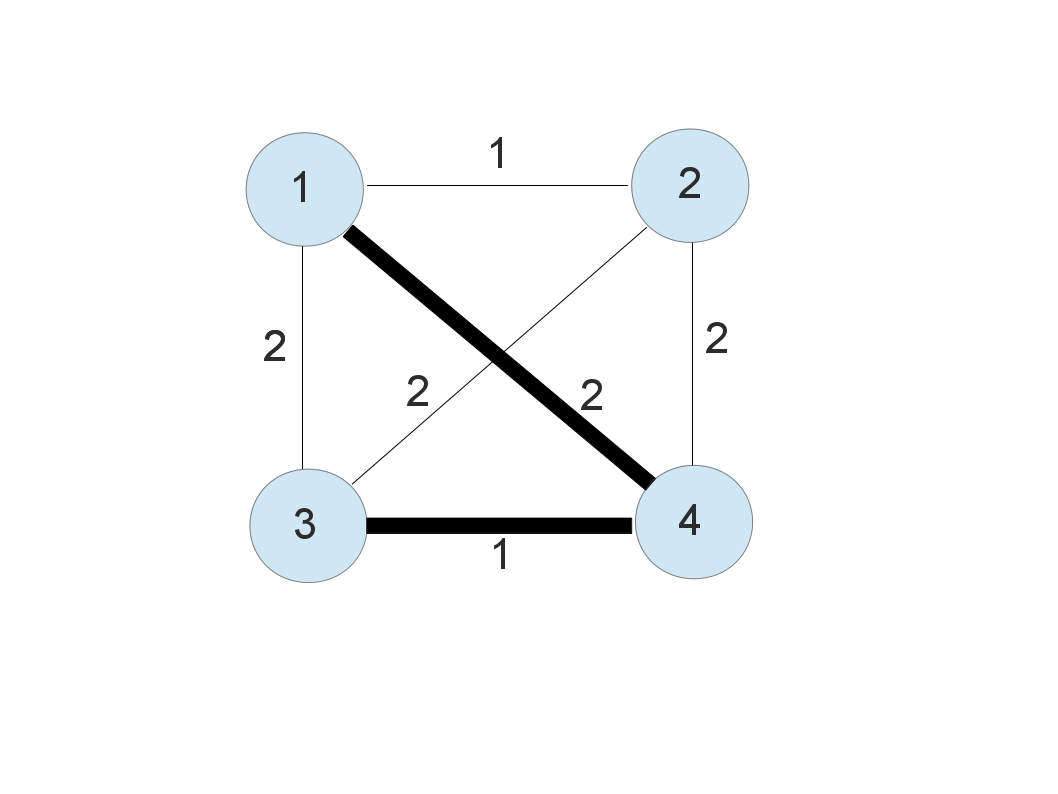
\includegraphics[scale=0.3]{ej3/imgs/graph_test2_sol.png}}
  \subfloat[Costo total: 12]{
   \label{}
    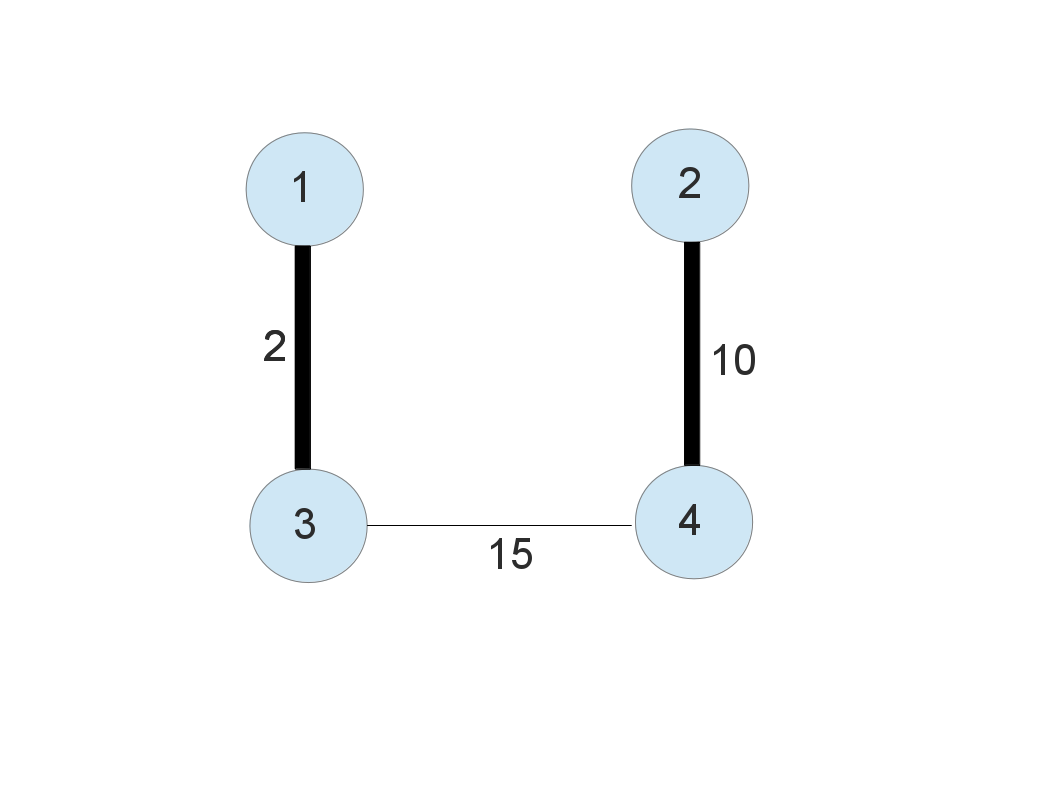
\includegraphics[scale=0.3]{ej3/imgs/graph_test3_sol.png}}
  \subfloat[Costo toal: 25]{
   \label{}
    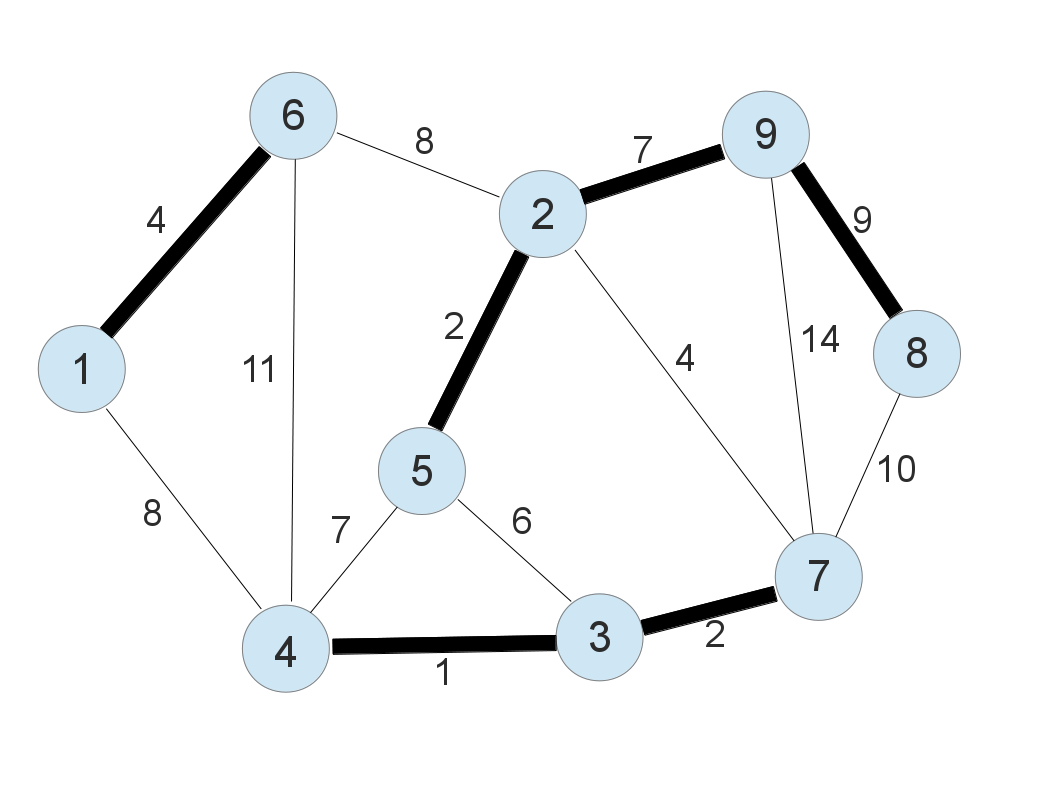
\includegraphics[scale=0.3]{ej3/imgs/graph_test4_sol.png}}
 \caption{Casos de prueba}
 \label{Soluciones halladas por el algoritmo}
\end{figure}

Las soluciones halladas son óptimas para los problemas presentados.
